\documentclass[11pt,letterpaper]{article}
\usepackage{amsfonts, amsbsy, amsmath}
\usepackage{graphicx}
\usepackage{cite}
\usepackage{url}
\usepackage[autostyle]{csquotes}
\usepackage[labelformat=simple]{subcaption}
\renewcommand\thesubfigure{(\alph{subfigure})}
\usepackage{fancyvrb}
\usepackage{hanging} % handging indent
\usepackage{booktabs}
\usepackage{makecell}
\usepackage{multirow}
\usepackage{hhline}
\usepackage{caption}
\usepackage{adjustbox}

% line arts
\usepackage{tikz}
\usetikzlibrary{shapes.geometric, arrows, positioning, shadows}

\usepackage{listings}
\lstset{
    basicstyle={\small\ttfamily},
    escapeinside={*@}{@*},
    breaklines=true
}
\usepackage{paralist}
\PassOptionsToPackage{hyphens}{url}\usepackage{hyperref}
\hypersetup{
    colorlinks,
    citecolor=black,
    filecolor=black,
    linkcolor=black,
    urlcolor=black
}

%
% added for accomodating long tables
%
\usepackage{longtable}
\let\oldlongtable\longtable
\def\longtable{\footnotesize\oldlongtable}


\usepackage{xr}
\externaldocument{report}\externaldocument{supplement/supplement}

%%%%%%%%%%%%%%%%%%%%%%%%%%%%%%%%%%%%%%%%%%%%%%%%%%%%%%%%%%%%%%%%%%%%%%%%%
%%%%%%%%%% EXACT 1in MARGINS %%%%%%%                                   %%
\setlength{\textwidth}{6.5in}     %%                                   %%
\setlength{\oddsidemargin}{0in}   %% (It is recommended that you       %%
\setlength{\evensidemargin}{0in}  %%  not change these parameters,     %%
\setlength{\textheight}{8.5in}    %%  at the risk of having your       %%
\setlength{\topmargin}{0in}       %%  proposal dismissed on the basis  %%
\setlength{\headheight}{0in}      %%  of incorrect formatting!!!)      %%
\setlength{\headsep}{0in}         %%                                   %%
\setlength{\footskip}{.5in}       %%                                   %%
%%%%%%%%%%%%%%%%%%%%%%%%%%%%%%%%%%%%                                   %%
%%%%%%%%%%%%%%%%%%%%%%%%%%%%%%%%%%%%%%%%%%%%%%%%%%%%%%%%%%%%%%%%%%%%%%%%%

\newcommand{\comment}[1]{\noindent \textbf{Comment. }{\em ``#1''}}
\newcommand{\response}[1]{\vskip 0.5em \noindent \textbf{Response. }{#1}}
\newcounter{reviewer}
\newcounter{comment}
\newcommand{\reviewerno}[1]{\setcounter{comment}{0}\refstepcounter{reviewer}\label{#1}}
\newcommand{\commentno}[1]{\refstepcounter{comment}\label{#1}}
\newcommand{\refcomm}[2]{{\em Comment R\ref{#1}.\ref{#2}}}

\newcommand\shortcite\cite

\makeatletter
\renewenvironment{table}%
  {\renewcommand{\familydefault}{\sfdefault}\selectfont
	  \@float{table}}
		  {\end@float}
\makeatother

\makeatletter
\newcommand*\my@starttable[1][]{%
	\@float{table}[#1]\footnotesize
	}
	\patchcmd{\table}{\@float{table}}{\my@starttable}{\PackageInfo{mysty}
	{Table environment patched successfully.}}
	{\PackageWarning{mysty}{Could not patch table environment.}}
\makeatother


\renewcommand{\mkbegdispquote}[2]{\ttfamily}

\newcommand{\code}{\texttt}

\newenvironment{revisiontext}
{
	\begin{flushright}
  \begin{minipage}{0.9\textwidth}\sffamily
}
{
  \end{minipage}
	\end{flushright}
}

\setcounter{section}{0}

\title{Revision Report for 
``Detecting Network-based Internet Censorship
  via Latent Feature Representation Learning''}
\author{Shawn P. Duncan and Hui Chen}
\date{\today}
\begin{document}
\maketitle
\tableofcontents
\vskip 3em

\noindent 
We thank the editor-in-chief and the associate editor for handling our paper in
a timely fashion. We owe a great deal of gratitude to the two anonymous
reviewers for their reviews of our paper. 
    
The reviewers pointed out strengths including novelty and contribution of our
paper.  We appreciate these encouraging comments.  The reviewers also indicated
several shortcomings in the paper.  In the following, we summarize our
revisions and our responses to the comments on the shortcomings.  For
convenience, we divided and numbered these comments of the two anonymous
reviewer, e.g., R1.1 is the 1st comment of reviewer \#1 while R2.1 that of
reviewer \#2.  We believe that we addressed and responded all comments on the
shortcomings from the two reviewers.  By addressing these comments we also
believe that we improved the quality of the paper. 




\reviewerno{r1}
\section{Responses to Reviewer \ref{r1}}

%%%%%%%%%%%%%%%%%%%%%%%%%%%%%%%%%%%%%%%%%%%%%%%%%%%%%%%%%%%%%%%%%%%%%%%%%%%%%%%
%                           Comment and Reponse                               %
%%%%%%%%%%%%%%%%%%%%%%%%%%%%%%%%%%%%%%%%%%%%%%%%%%%%%%%%%%%%%%%%%%%%%%%%%%%%%%%

\commentno{r1bm}
\subsection{\refcomm{r1}{r1bm}. On Baseline Model}

\comment{%
How realistic is the baseline model used for comparison? Is it being used in
	the industry or proposed by prior work?%
}
\response{
	This is a great question. To the best of our knowledge, our work is the first work 
	that presents an end-to-end automatic Internet censorship detection model. As such,
	a baseline model is not readily available. 

	In order to construct a baseline model, we examined the literature.
	We realized that researchers generally rely on rule-based
	detection methods, sometimes assisted with machine learning algorithms, most of those
	are unsupervised. One example is Niaki et al. who compute page length and 
	term-frequency as data features for each 
	Internet outage response page, cluster the response pages into clusters, and manually examine
	the clusters~\cite{niaki2020iclab}. Another is Raman et al. who encode each Internet response
	page as an image, and use image clustering algorithms to automatically cluster the pages~\cite{raman_measuring_2020}. 

    The motivation for Raman et al.~\cite{raman_measuring_2020}'s image-based data feature 
    representation came from several studies that found the page-length and term-frequency 
    features lead to high false positives for censorship detection~\cite{yadav2018light, 
    raman_measuring_2020}. Raman et al.'s work shows that the image-based feature
    representation yields an improved censorship detection performance in their approach
    combining clustering and manual inspection.
    

	Following the prior works, we design and propose an image-based detection model as
	the baseline model. The feature representation part is identical to that in Raman et al.~\cite{raman_measuring_2020}.
	Upon extracting the features, we use a simple classifier (a multi-layer neural network) to classify the
	response pages. For our autoencode-based end-to-end model, we design an autoencode network to extract
	features, while keeping the classifier identical to the baseline model.

	Considering the above, we believe our baseline model is well justified. To reflect on this justification,
	we revised ``Section 3.4 Alternative Approach'' as follows:
}

\begin{revisiontext}

	Prior works typically adopt a semi-automated approach for Internet censorship 
	detection, where they first leverage an unsupervised machine learning algorithm,
	such as, a clustering algorithm to divide Internet outage measurements, e.g.,
	block pages into clusters, and second, manually examine the clusters to determine
	whether the cluster represents a type of Internet 
	censorship~\cite{raman_measuring_2020, niaki2020iclab}. A necessary step
	in the process is to extract data features from the internet
	measurement data. Page length and term frequency vectors are two features
	borrowed from natural language processing to cluster block 
	pages~\cite{jones2014automated}. Although the clustering algorithm
	using the two features reduces manual efforts to examine the clusters,
	several follow-up studies indicate that the features can lead to 
	high false positives due to natural variations in page length from dynamic
	and language-specific content~\cite{yadav2018light, raman2020measuring}. 
	Recognizing the limitation of the two features, researchers are seeking 
	different feature representation methods for Internet measurement data, such as,
	block pages~\cite{raman2020measuring}.
	
\end{revisiontext}
\vskip 0.5em
\begin{revisiontext}
			
	
	Deep learning has found tremendous success in computer
	vision~\cite{huang_densely_2017, li_fei-fei_imagenet_2012}. In contrast to 
	more traditional learning algorithms, such as, Super-Vector Machine and 
	Tree-based algorithms (Decision Tree, Random Forest) for which we need to
	extract from the raw data manually designed features to represent the data
	in a tabular form, deep learning can learn to extract features directly
	from the raw data, which, numerous studies show it is an advantage because
	we do not always know what the best features might be for a particular 
	machine learning application~\cite{bengio2013representation}. 
	A clever way to
	design a learning system for non-tabular data is to take
	advantage of these recent advances in deep learning by encoding the data as
	gray-scale images and use a deep learning model for computer vision that is
	readily available to learn
	from these images. There have been applications of this approach in several
	domains, such as, for malware detection~\cite{hemalatha_efficient_2021} and for
	software defect prediction~\cite{chen2020software}.  A gray-scale image can be
	encoded using a byte pallet, in which the range from black to white is encoded
	as an integer between 0 and 255. In another words, we can consider a gray-scale
	image as a vector of $W \times H$ integers where $W$ is the width of the image
	and $H$ the height. For our structured data, after converting a
	censorship test record similar to that in Listing~1 into a
	raw vector, we pad the
	beginning and end of the vector with sufficient 0 to 
	equal a uniform length of size $W \times H$. We then export this vector to a
	sequence of bytes, reshape the vector to a $W \times H$ array from which we
	form the gray-scale image.
	
\end{revisiontext}
\vskip 0.5em
\begin{revisiontext}


	Recently several works
	have adopted this approach in their semi-automated censorship detection
	pipeline and find that the approach leads to improved predictive performance
	than those using the page length and term frequency vector 
	features~\cite{raman2020measuring, sundara_raman_censored_2020}. 
	Following these prior works, we build a fully-automated Internet censorship detection model
	where we use images as feature representations of block pages. For this,
	we elect to use the well-known DenseNet
	model~\cite{huang_densely_2017}.  DenseNet uses the architecture of a Convolutional
	Neural Network (CNN). A DenseNet has multiple CNN blocks that have the
	following neuron connectivity pattern: each layer in the CNN block
	is connected to all the others with the block. Due to this connectivity
	pattern, there is a shortcut path between each individual layer to the loss
	function and the training of the layer can be directly supervised by the loss
	function. Aside from this, the connectivity pattern also results in a compact
	network that is less prone to overfitting and encourages heavy feature reuse.
	Because of this, prior work suggests that DenseNet should be a natural fit for per-pixel
	prediction problems~\cite{zhu2017densenet}.
	
\end{revisiontext}
\vskip 0.5em
\begin{revisiontext}

	
	DenseNet is available as a pre-trained model~\cite{pytorchdensenet} 
	that expects images sized $224 \times 224$. The pre-trained model has a final linear
	layer of size 1,000 as a classifier for 1,000 image categories.  We replace
	that linear layer in the pre-trained model with a new layer accepting the same
	input dimension but producing a single output, the probability at which 
	the input is a censorship event.  
	
\end{revisiontext}
\vskip 0.5em
\begin{revisiontext}


	As an alternative to for the proposed End-to-End
	Censorship Detection model (E2ECD), we consider a modeling pipeline as
	illustrated in Figure~2b. For convenience, we refer to
	this model as DenseNetCD. Because the alternative model leverages the feature presentation method
	that prior works consider the best and is equipped with an identical classifier as the
	E2ECD model, we shall use it as a baseline model to compare
	with the E2ECD model. 
\end{revisiontext}

\commentno{r1fi}
\subsection{\refcomm{r1}{r1fi}. On False Identification (Positives and False Negatives)}

\comment{%
Do you explore the data records that are incorrectly identified as censored
	events by the proposed model? And/Or the censored records that are identified
	as normal?%
}
\response{
	This is an excellent question. Perhaps, most relevant is the discussion in 
	``Section 4.5. Censorship Detection on Undetermined Records''. For this, we did
	take a sampling approach, and randomly select several instances in each category
	to gauge its correctness. In the paper, we argue based on our examinations of
	the random samples:

	``Most of the remaining records are likely the result of censorship.  
	An investigation on the
	Great Firewall of China indicates that both \textit{connection reset by peer}
	and \textit{connection timed out} are among its observable
	characteristics~\cite{shu_data_2014}.  As discussed in the above, 
	the response to the request sent to
	these vantage points have been verified with innocuous payloads, and therefore
	it is very unlikely that the network has unexpectedly and repeatedly failed
	during these specific queries.''

	To have concrete understanding about the correctness or the incorrectness of the 
	prediction results, we need to infer both the detection mechanism and the censorship
	intention, which is a task of significant undertaking. Because of this, to make this
	clearer, we added the following paragraph to ``Section 5 Limitations and Threats to Validated''
	under ``Censorship Detection on Undetermined Test Records'':



}

\begin{revisiontext}
	Because the evaluation data set contains in total 842,842 records, a thorough
	examination of the prediction results manually is infeasible. We plan to study
	these test records in a future work. Because we are unable to access people's intention
	who might initiate the censorship events, the correctness of censorship 
	detection is often via cross-examination and inference. For this, we plan to
	compare records collected by multiple Internet censorship measurement 
	platforms including both the Censored Planet and 
	ICLab in the same time period~\cite{sundara_raman_censored_2020,niaki2020iclab}. 
	Second, following the approach adopted by prior works, we shall cluster
	the test records, such as, those predicted as probable censorship events, 
	and manually examine each cluster to determine whether the prediction is correct
	by inferring what the censorship mechanism is and what intention 
	of censorship may be~\cite{jones2014automated,sundara_raman_censored_2020,niaki2020iclab}. 
\end{revisiontext}


\reviewerno{r2}
\section{Responses to Reviewer \ref{r2}}

%%%%%%%%%%%%%%%%%%%%%%%%%%%%%%%%%%%%%%%%%%%%%%%%%%%%%%%%%%%%%%%%%%%%%%%%%%%%%%%
%                           Comment and Reponse                               %
%%%%%%%%%%%%%%%%%%%%%%%%%%%%%%%%%%%%%%%%%%%%%%%%%%%%%%%%%%%%%%%%%%%%%%%%%%%%%%%

\commentno{r2mv}
\subsection{\refcomm{r2}{r2mv}. On Motivation}

\comment{%
	To strengthen the motivation of the paper, it would be appropriate to address
	the doubts and preconceptions that a reader who is not familiar with
	censorship might have. For instance, most people would assume that a
	democratic country would rarely apply censorship and if it does, with a
	warrant, it would inform about that. If that were true, why would not simply
	rely on a country or set of `free' countries as the basis for detection?%
}
\response{
	That is an insightful observation. Following this advice, we revised/added several sentences to the Introduction section.
	The relevant text now reads as follows:
}

\begin{revisiontext}
	The network-based Internet censorship can lead to network
outages~\cite{dainotti2011analysis}.  Differentiating the censorship events
from other types of outages can thus benefit the design and implantation of
Internet network architecture, protocols, and
systems~\cite{aceto2018comprehensive, aceto_internet_2015}.  Understanding the
censorship mechanism can also help develop circumvention
techniques~\cite{winter2012great, chai2019importance, satija2021blindtls}.
\vskip 0.5em
Aside from these technical perspectives, there have been pursuits to gauge its
social, political, cultural, and religious
implications~\cite{shishkina2018internet, meserve2018google,
chen2000pornography}. These works reveal the complexity and the intricacy of 
the Internet censorship, which sometimes challenges conventional wisdom
given its prevalence among countries, polities, cultures, and religions 
of a great spectrum~\cite{aryan2013internet, nabi2013anatomy, singh2017characterizing,
yadav2018light, ng2018detecting,
meserve2018google, bock2021even, padmanabhan2021multi, ververis2021understanding}.
\end{revisiontext}

\noindent
	Internet censorship is a complex global phenomenon. It can be argued that in democratic
	countries Internet censorship may be less frequent than in non-democratic countries; however, it is
	certainly an overstatement to insist that there is no Internet censorship in democratic
	countries. Figure 8 in Niaki et al. clearly exhibits this~\cite{niaki2020iclab}.
	Meserve and Pemstein provide an investigation on Internet censorship in democratic
	countries with an aim to answer the question, ``how do democracies censor the internet,
	and why?~\cite{meserve2018google}'' Censored Planet~\cite{sundara_raman_censored_2020} queries the endpoints around the globe both for these reasons and for comparison.
 
    Arguably, there are more peer-reviewed studies
	about Internet censorship in non-democratic countries where Internet censorship is
	more prevalent. These studies include multiple studies on
	the Great Firewall of China, on Internet censorship in Iran, Myanmar, and Pakistan, 
	and on censorship mechanisms
	adopted in these countries~\cite{aryan2013internet, nabi2013anatomy, singh2017characterizing,
	ng2018detecting, bock2021even, padmanabhan2021multi}. 

	However, the censorship phenomenon is too complex
	for us to give a fair treatment in this article. Rather, this article is on automatic detection techniques
	of Internet censorship. The aim here is to investigate methods that could provide better tools to keen "observers." 


\commentno{r2xmlr}
\subsection{\refcomm{r2}{r2xmlr}. On Application of XLM-R}

\comment{%
A figure might clarify the approach based on XLM-R that is used to encode the
	text fields.%
}
\response{
	In Section 3.1, we added a figure to the paper in order to make the description of the tokenizer clearer. The added text and figure 
	are as follows:
}

\begin{revisiontext}
		Figure~\ref{fig:xlmr} illustrates the processing pipeline
		for these data fields. 

		\vskip 1em

		% \begin{figure}[!htbp]
			\centering
			\begin{adjustbox}{max width=\textwidth}
			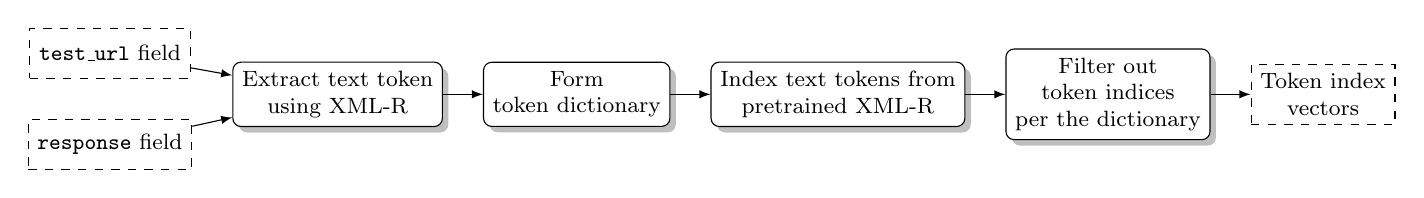
\begin{tikzpicture}
				\tikzset{
					node distance=0.2in and 0.2in,
					inout/.style={rectangle, draw, dashed, black, align=center, font=\footnotesize,
					minimum height=0.25in, rounded corners=0pt},
					box/.style={rectangle, draw, solid, black, drop shadow, fill=white, align=center, font=\footnotesize,
					minimum height=0.25in, rounded corners=3pt}
				}
				\node[inout](url){\code{test\_url} field};
				\node[inout, below=of url](resp){\code{response} field};
				\node[box, right=of resp, yshift=0.25in](token){Extract text token\\using XML-R};
				\node[box, right=of token](dict){Form \\ token dictionary};
				\node[box, right=of dict](xmlr){Index text tokens  from\\pretrained XML-R};
				\node[box, right=of xmlr](filter){Filter out\\token indices\\per the dictionary};
				\node[inout, right=of filter](vector){Token index \\vectors};
		
				\draw[-latex](url) -- (token);
				\draw[-latex](resp) -- (token);
				\draw[-latex](token) -- (dict);
				\draw[-latex](dict) -- (xmlr);
				\draw[-latex](xmlr) -- (filter);
				\draw[-latex](filter) -- (vector);
		
				
			\end{tikzpicture}
			\end{adjustbox}
			\captionof{figure}{\sffamily Multilingual data processing of the \code{test\_url} and \code{response} fields and dimensionality reduction via 
			a pretrained XLM-R model~\cite{conneau2020unsupervised}. 
			The \code{response} field can contain natural language text and program code. To reduce the size of the encoding vectors, We
			filter out those with low frequency, such as, those do not appear in our data (i.e., frequency is 0) or rarely appear depending
			on the constraint of the available computational resources. In this work, by filtering out tokens with frequency of 0, we reach
			sufficiently small embedding vectors of length of 6,813.}
			\label{fig:xlmr}	
			
		% \end{figure}
	\end{revisiontext}


\commentno{r2ct}
\subsection{\refcomm{r2}{r2ct}. On Context Vector of the Model}

\comment{%
	Please describe in further detail the context vector.%
}
\response{
	This is great advice. In Section 3.2, we added the following sentences and revised the discussion about the attention score as follows:
}
\begin{revisiontext}
	$\ldots$

	$\ldots$
The weighted context vector here is to capture
the importance of different source-side information (e.g., which element in the state
vector) for predicting the probability of a particular token in the vocabulary~\cite{luong2015effective}.
We shall give a more detailed treatment of the context vector below (See the discussion about  Equation~\eqref{eq:attention}).
	$\ldots$

	$\ldots$

	The decoder is a sequence of bidirectional Gated Recurrent Unit Cells. We enhance
	it with an attention mechanism~\cite{niu2021review}, in particular, the ``dot'' 
	attention mechanism~\cite{luong2015effective}. 
	Instead of using fixed
	neuron weights, the attention mechanism allows us to enhance the 
	effect of some parts of the input data while diminishing other parts for predicting
	token probabilities via attention scores. 
	In one
	direction, each token in the input sequence is processed through the GRU cells.
	In the other direction, we calculate attention scores. Attention scores are
	computed using a dot product~\cite{raff_inside_2021}
	
	\begin{equation} \label{eq:attention}
	score(h_t, c_t) = \frac{h_t^T \cdot c_t}{\sqrt{H}}
	\end{equation}
	
	\noindent with values of $h_t$ taken from the state produced at step $t$ by the
	encoder, $h_t^T$ is $h_t$'s transpose, $c_t$ is the context, 
	and $H$ is the
	input size used for the GRU Cell. We compute $c_t$ as the decoder output at step $t$.
	We use the attention scores to weight the input sequence at each step of the decoding process.
	
\end{revisiontext}	

\commentno{r2bm}
\subsection{\refcomm{r2}{r2bm}. On Baseline Model}

\comment{%
	It would be interesting to use another simpler approach as the baseline
	method to assess how typical/naive classifier methods would perform in this
	problem. Although the comparison with image classification is useful, a
	naiver approach would serve better to the purpose of motivating the need for
	the complex combination of techniques that are proposed (i.e., the need for
	representation learning, sequence encoding, etc.).%
}
\response{
	This is an excellent suggestion. Typically, to use a simple model, we need
	to construct tabular data from the Internet measurement data where each column 
	is a data feature and each row is a feature vector for the corresponding 
	measurement record. 

	The tabular data are not readily available. We must decide what features to 
	construct and extract from the measurement data. By comparing existing features, 
	the best performing features in prior works are the image representation of 
	the measurement records~\cite{raman_measuring_2020, niaki2020iclab}. 
	In our baseline model, we adopt the image representations
	of the measurement records extracted using a pretrained neural network. Typically,
	neural networks are adopted as a classifier for the image data~\cite{hemalatha_efficient_2021,chen2020software}. 
	Our baseline model is built upon this. As such, we believe that a simple baseline
	model, such as, a Random Forest model using the features like page length and 
	term frequency vectors are unnecessary since these features are already shown to
	yield large false positives in prior researches on Internet censorship 
	detections~\cite{yadav2018light, raman2020measuring}. 
	
	In our response to Review~\ref{r1}'s comment~R\ref{r1}.\ref{r1bm}, 
	we have a detailed discussion about the baseline model. We hope our responses are
	adequate to address the reviewer's concern. 




}



\bibliographystyle{plain}
\bibliography{paper}
\end{document}
